\documentclass[10pt]{exam}
\usepackage[phy]{template-for-exam}
\usepackage{tikz}
\usepackage[top=0.2in, bottom=0.5in, left=1in, right=1in]{geometry}


\begin{document}
\pagestyle{empty}

\def\mytitle{Unit 08 Test: SHM}

\newcommand{\topmatter} {
  \vspace{2em}
  \hrule

  \vspace{1em}

  \section*{Equations}

  \begin{align*}
    T_P &=2\pi\sqrt{\frac{\ell}{g}} &
    T_S &=2\pi\sqrt{\frac{m}{k}} &
    F_S &= -kd &
    F_G &= mg  &
    v   &= f\lambda & &&
    g   &= \SI{9.8}{m/s^2}
  \end{align*}

}
\newcommand{\bottommatter}{

}

\newcommand{\drawscantron}[2]{
  \begin{flushright}
    \begin{tikzpicture}
      \node[anchor=south west] at (0,0) {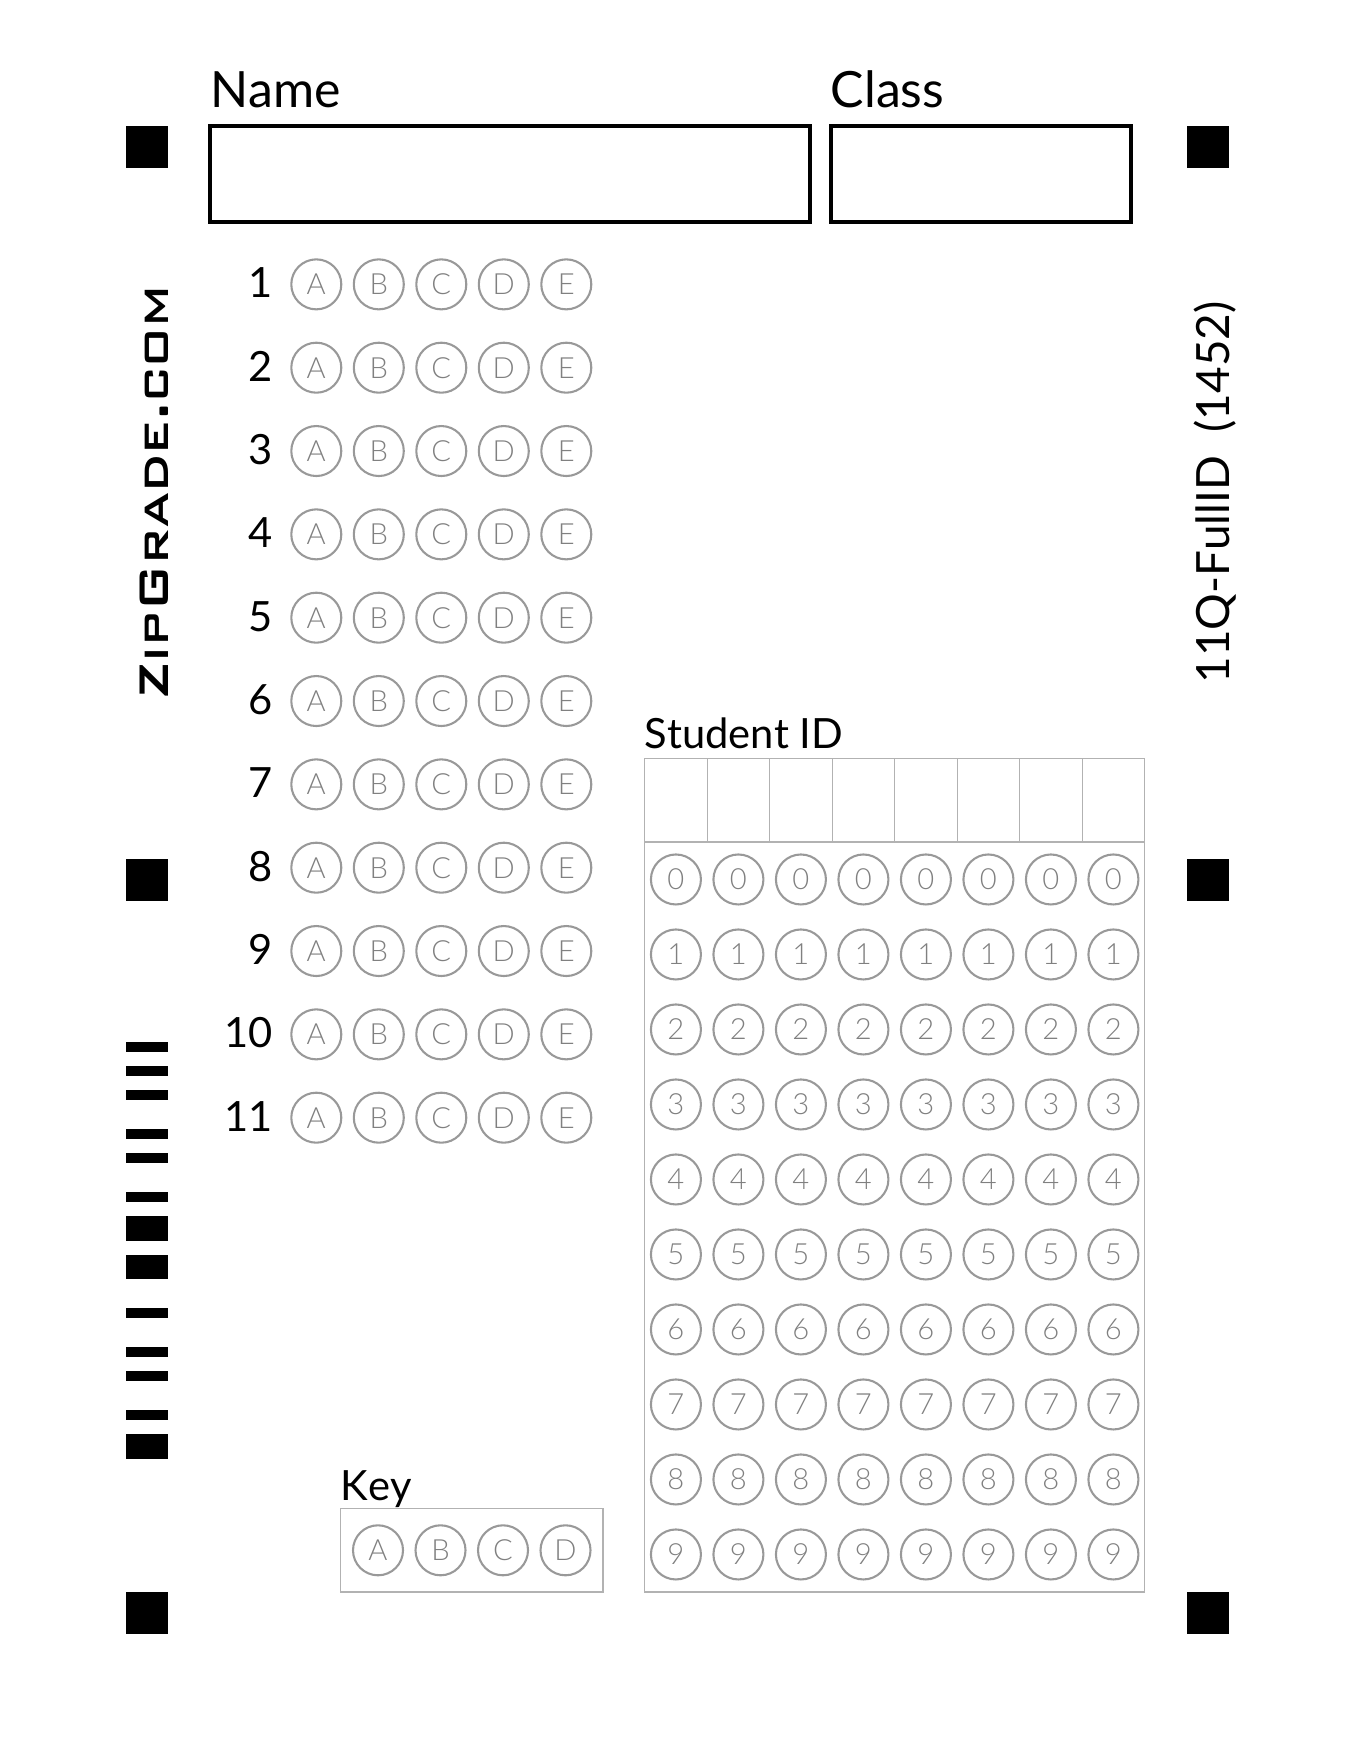
\includegraphics[width=4in]{11Q.png}};
      \fill (#1,#2) circle (0.2);
    \end{tikzpicture}
  
    \bottommatter
  \end{flushright}
}



  \drawscantron{2.95}{1.7}
  \topmatter

\pagebreak

  \drawscantron{3.4}{1.7}
  \topmatter

\pagebreak

  \drawscantron{3.86}{1.7}
  \topmatter

\pagebreak

  \drawscantron{4.35}{1.7}
  \topmatter


\end{document}